\documentclass{document_layout}

% Title and author information 
\title{METROLOGY WITH SYNTHETIC FRINGE PATTERNS FOR THREE DIMENSIONAL SCANNING AND RECONSTRUCTION}
\author{
    Eduardo Barroso \address{1} and Alexandre Sauze \address{1} \\[0.3em]
    {\scriptsize
        \address{1} Department of Physics Engineering; Monterrey Institute of Technology, Monterrey, N.L 64849.\\
    }
}
\date{December, 2022}

\setabstract{
    As of 2021, the digital revolution has shaped every industry thanks to the ever growing computational power accessible to the population. 
    Thus, being able to digitally extract and process data has become a key virtue in many business worldwide. 
    In this work, we aim to illustrate the working principles of a digital scanning technology called Moire by fringe displacement.
    The team shows that with a projector, camera and a computer; it is possible to measure the depth of a 3D system. 
    This has applications in diverse fields like: quality control, biomedical, archaeology and the fashion industry.
    }

% Begin the document
\begin{document}

\maketitle

\section{Introduction}
\label{sec:INTRO}

Photography works by capturing different light intensities of a frame limited by the lens of the camera. Similarly, holographic technologies are able to capture the intensity and phase of the light being reflected off a 3D surface. This phase can be seen as extra information about the object and therefore gives the illusion of depth when the hologram is generated. In a similar way, it is possible to measure three dimensional depth by studding how a set of sinusoidal fringes deforms when projected onto a 3D geometry \cite{gaasvik2003optical}. The fringe deformations are encoded into the phase of the fringe pattern. By decrypting such phase, it is possible to measure the topography of the geometry being scanned. This techniques is known as Moiré by fringe displacement and its of of the many techniques studied by the field of optical metrology.  \\

This work aims to present a methodology that exploits Moire by fringe displacement to reconstruct a three dimensional bust using available market technology. The principal tools to implement this metrology are: a light source, a camera, a reference screen and of course; a computer. Furthermore, the team believes that with minor modifications to the methodology presented, this technology can have applications in the field of medical imaging, fashion industry, paleontology and archaeology \cite{Schofield:03}. Given that a person knows the technology and has access to the tools listed below; it is possible to obtain three dimensional measurements of a irregular geometry. Furthermore, these digital measurements can later be processed by computers including artificial intelligence algorithms. \\

Like any other technology, there are some limitations to what can be done with this technique of optical metrology. The considerations to this limitations are also exposed in the work. Thus, the purpose of this work is limited to understanding the key elements behind this technology to further propose upgrades, generalizations and concrete applications. To do so, the team scans and reconstructs computationally an interesting geometrical object. \\


\section{Theoretical Framework}
\label{sec:TEO_FRAMEWORK}
%%%%%%%%%%%%%%%%%%%%%%%%%%%%%
When a phase is introduced to an harmonic system by a source, information about this source is encoded into the patterns. Some holographic technologies use this extra information to generate three dimensional depth perception \cite{gaasvik2003optical}. Furthermore, it is possible to extract quantitative measurements of the size of the source by quantifying the alterations in the patterns. The branch of science that deals with such problems is optical metrology\cite{Zhang:07}. \\

In this work, we will use synthetic fringe patterns to scan a bust shown in figure \ref{fig:Bust} and then obtain quantitative data. These scans will be stored in a series of 4 photographs that are later subjected to a data processing model that will yield out of plane measurments. This model is known as Moire by fringe displacement. 

\subsection{MOIRE BY FRINGE DISPLACEMENT}
The Moire effect was first mentioned as a stress or deformation identifying technique in 1954 by John Guild from the National Physical Laboratory, however this technique may have been used before the last century \cite{creath1992moire}. The Moiré effect can be very effective in showing stress and deformation in any engineering piece or material as it is highly sensitive to variations. \\ 

Moire by fringe displacement consists on capturing a set of photographs where the fringes scanning the object displace a integer multiple of $2\pi/n$, where n is the number of pictures. Studies \cite{creath1992moire} show that more pictures is related to more detail and less pictures yield faster computational results. For the case of this study, the team uses 4 step fringe displacement. Thus, each photograph will correspond to a intensity profile described by one of 4 equations:
\begin{align}
    I_1 &= I_A + I_B + 2\sqrt{I_AI_B} cos(\phi),\\
    I_2 &= I_A + I_B + 2\sqrt{I_AI_B} cos(\phi + \pi/2),\\
    I_3 &= I_A + I_B + 2\sqrt{I_AI_B} cos(\phi + \pi),\\
    I_4 &= I_A + I_B + 2\sqrt{I_AI_B} cos(\phi) + 3\pi/2,
    \label{eq:system_of_I}
\end{align}
 
where, $\phi$ is the phase that encodes the quantitative measurements. 

\subsection{PHASE}
The technique starts with a reference set of synthetic sinusoidal fringes generated by a projector. Later, this technique measures a displacement in the fringes deformed by the object. This displacement is encrypted onto the phase $\phi$ of the system. This gives a way to mathematically quantify such information  \cite{gaasvik2003optical}. Few geometrical relations are implemented to solve the system of equations ((1) to (\ref{eq:system_of_I}))  for $\phi$ to obtain that 
\begin{equation}
    \phi = atan(\frac{I_4-I_2}{I_3-I_1}).
    \label{eq:phase}
\end{equation}
Computationally, this means operating with four pixel matrices $I_n$ to obtain a matrix that at each pixel has a phase defined by equation \ref{eq:phase}. However, because of the nature of the $atan$ function, the phase will have discontinuities. It is said that the phase is wrapped between $[-\pi, \pi]$. This means that in unknown indices, the phase will have discontinuities of $2*\pi$ as shown in figure \ref{fig:WRAPunwrap}.\\


\subsection{UNWRAPPING}
In mathematics, this is called the wrapped phase problem. The unwrapping consists on finding discontinuities within the phase and adding a correcting factor of $2*pi$ to unwrap the phase\cite{Huntley:93}\cite{Ghiglia:94}. This task is more complex that it seems at first sight. Take figure \ref{fig:Bust} containing 121,959,936 pixels, add some noise due to experimental considerations and try to unwrap its phase with arithmetic, ordered and efficient operations. 

\begin{figure}[H]
    \centering
    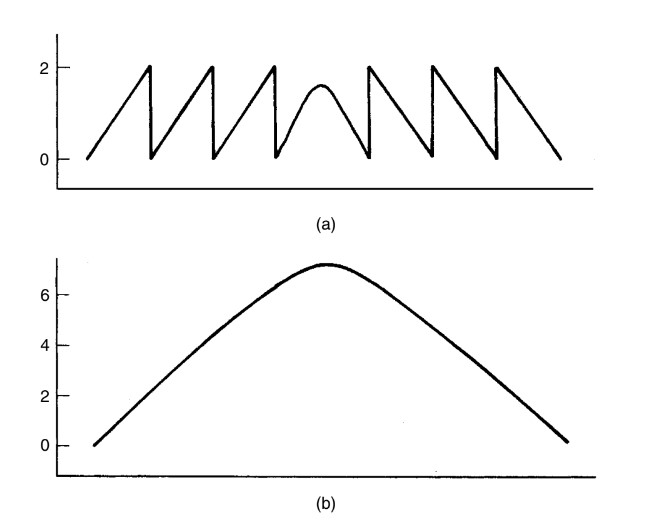
\includegraphics[width=0.25\textwidth]{Figures/UnwrappIlustration.jpg}
    \caption{(a) 'Saw-tooth’ wrapped phase function. (b) Phase function obtained by ‘unwrapping’ (a) \cite{gaasvik2003optical}}
    \label{fig:WRAPunwrap}
\end{figure}


\subsection{THREE DIMENSIONAL IMAGE RECONSTRUCTION}
After unwrapping is implemented successfully all is left a pure phase. This phase has encoded the depth measurements of the scanned object but also encodes information about the experimental parameters. In particular the angles formed by the camera and the scanned object $\beta$ (Figure \ref{fig:Exp_Setup}) and the spatial frequency of the fringes $w$.
%%FIGURA DE BETA Y W
In order to consider the experimental parameters in this model, Moire by fringe displacement puts forward a geometric relation between the phase $\phi$ and the topography of the object $z(x,y)$. Using 
\begin{equation}
    z = \frac{\phi}{2\pi} \frac{w}{tan(\beta)},
    \label{eq:topography}
\end{equation}
it is possible to decript the quantitative measurement of the scanned object. At any point of the scan, this technique will assign a z value. This information is stored in a matrix with dimensions specified by the photographs. 

% The beauty is in its simplicity. 
% Clever algorithmic implementations in Matlab
% Pasting two surfaces


\section{Results}
\label{sec:RESULTS}
In section \ref{sec:INTRO}, we discussed the principal fields that can benefit from optical metrology. In order to encompass the majority of the fields in the experimental section, the team decided to reconstruct a polystyrene bust as shown in figure \ref{fig:Bust}.
\begin{figure}[H]
    \centering
    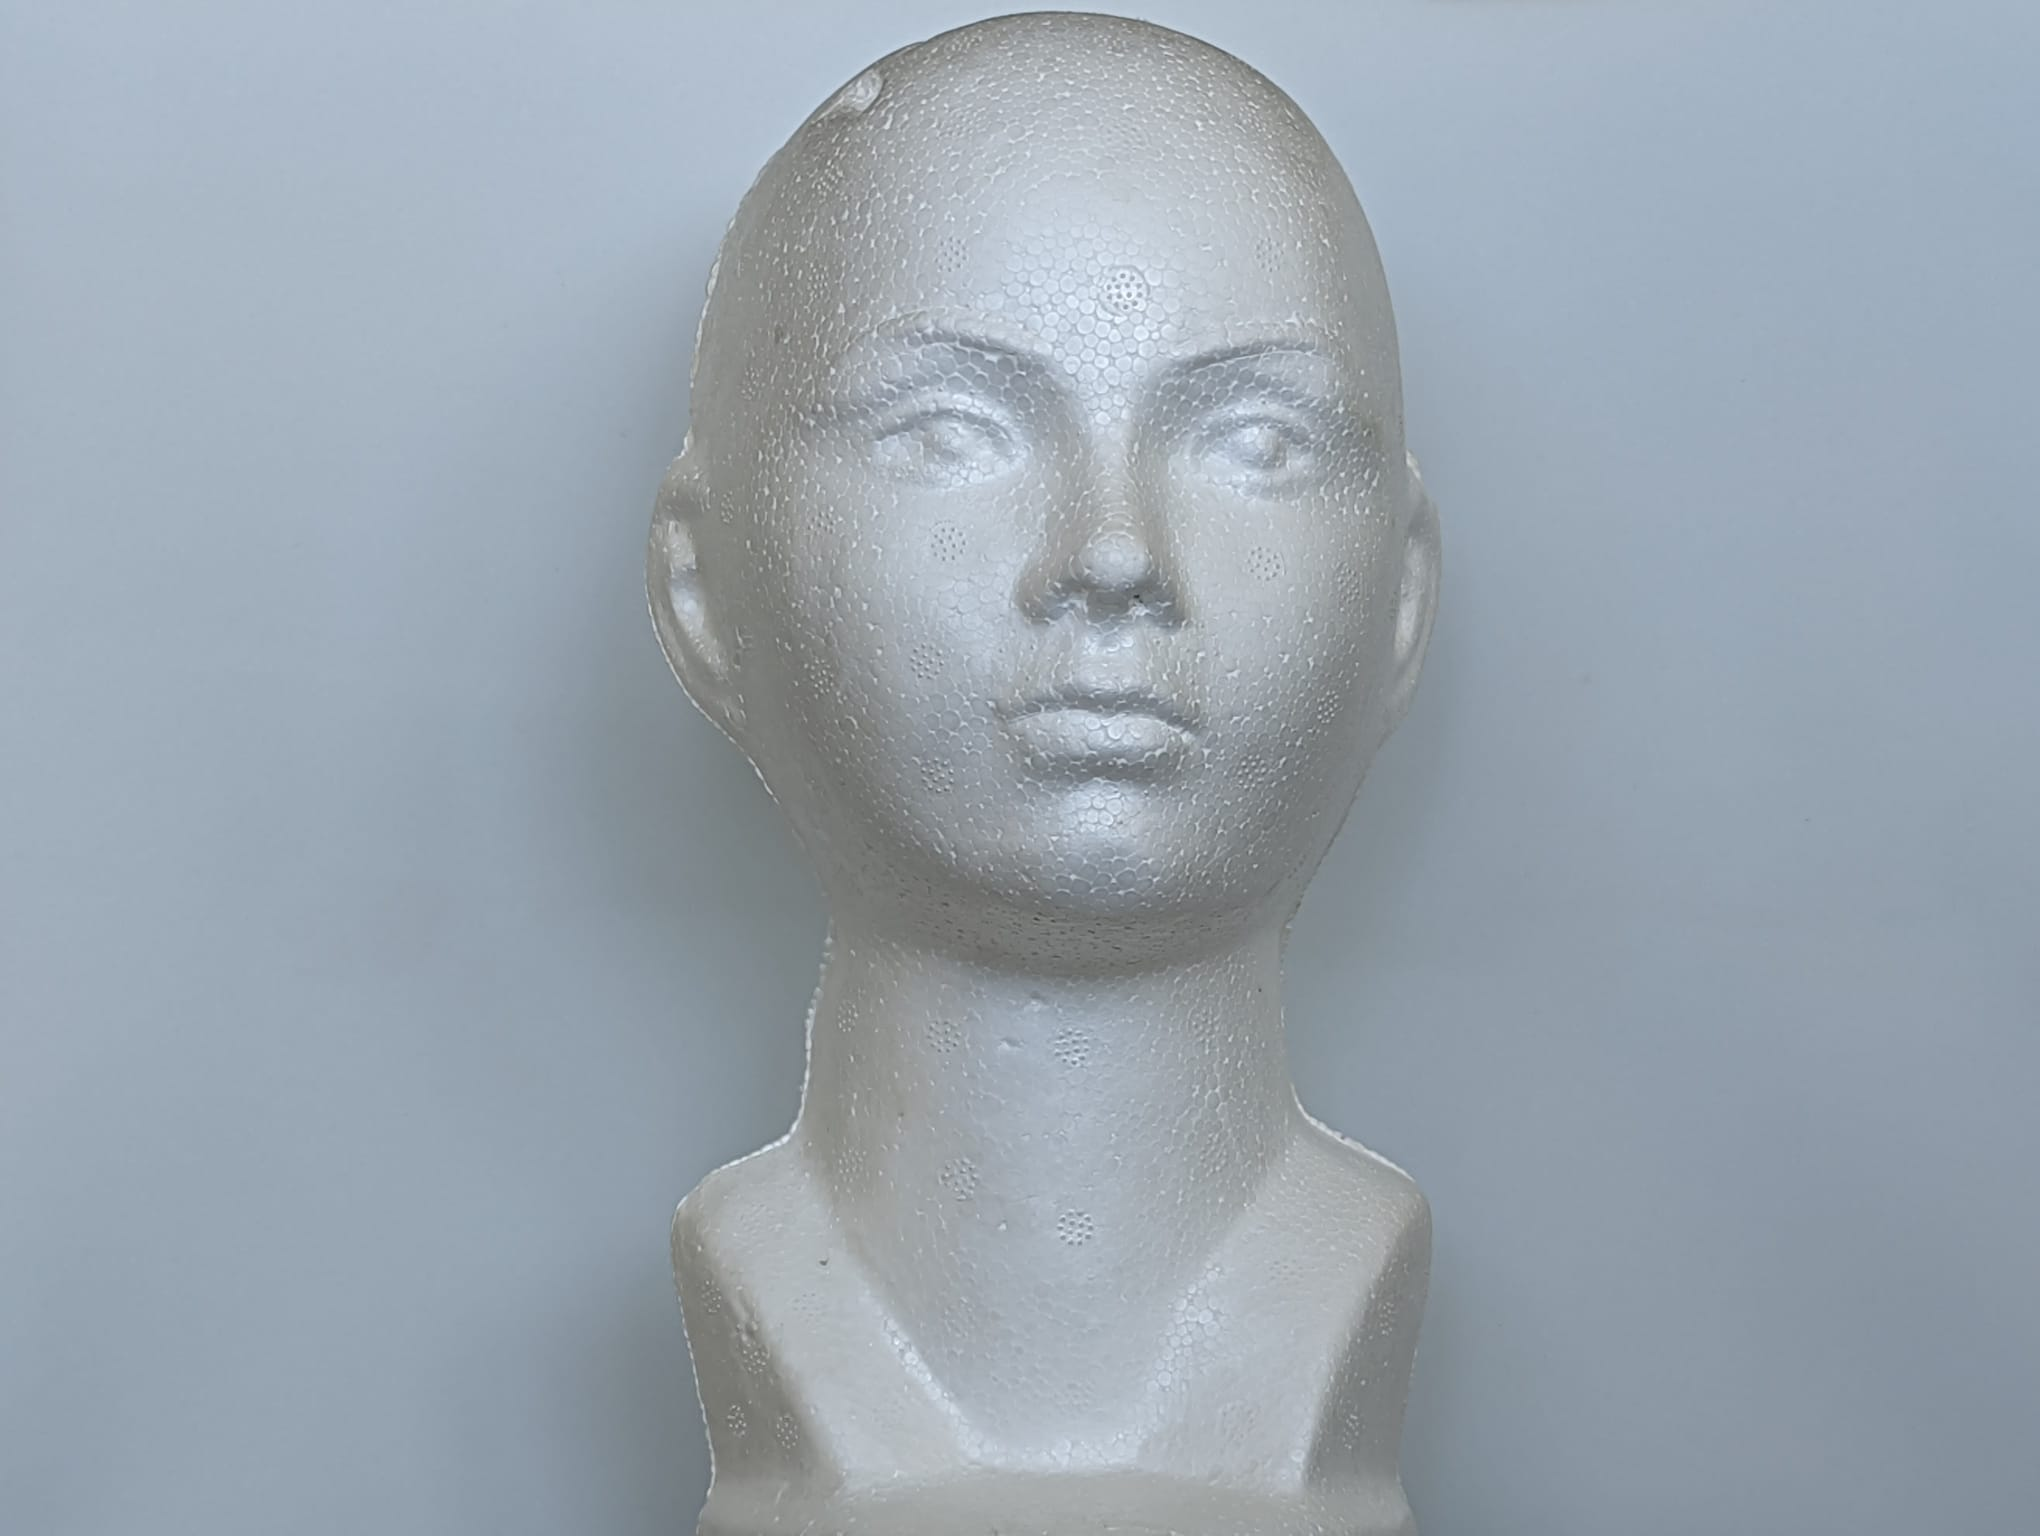
\includegraphics[width=0.3\textwidth]{Figures/Plain_Bust.jpeg}
    \caption{Polystyrene Bust}
    \label{fig:Bust}
\end{figure}

\subsection{SYNTHETIC FRINGES}
It can be shown that optical interference generates sinusoidal fringe patterns. Furthermore, by introducing different polarization's in a beam´s transversal profile it is possible to displace the fringes between zero and $2\pi$. This is done by using a linear polarizer to pick the different polarized states giving the illusion of fringe displacement. Implementing a scanning system like this means that you need an optical arrangement with highly controlled conditions and this is not aligned with the work´s goal. For this reason, the team used synthetic fringes generated by a conventional projector. \\

\begin{figure}[H]
    \centering
    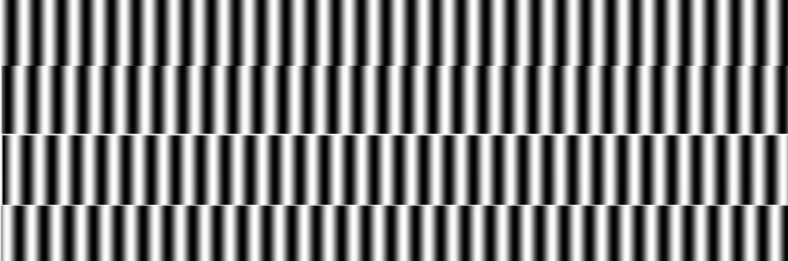
\includegraphics[width=0.4\textwidth]{Figures/Fringe_Disp.jpg}
    \caption{Synthetic Fringes}
    \label{fig:Fringe_Disp}
\end{figure}

Other advantages of using synthetic fringes is the greater control they offer. In particular we are intrested on the orientation, contrast and the spatial frequency ($w = 0.6 cm$). To implement such fringes, the team used the licensed software MATLAB to generate a video that includes the 4 frames of the displaced fringes (Figure \ref{fig:Fringe_Disp}). This video is then uploaded to the projector to further be projected in a scanning session. \\ 

\subsection{EXPERIMENTAL SETUP}
%Fondo blanco mate plano
%Remover ruido exterior
%Fijar puntos para instalacion de busto
%Considerar altura de enfoque
%Parametros experimentales \beta y w

For the experiment, the projector and the nose of the mannequin were adjusted to the same heights at a distance of roughly 1.53 meters of separation between both elements, this distance ensured that the focal point of the projection was at the same level as the ears to guarantee a similar quality of image between the front of the face and the background. The camera was placed below the projector's lens at 1.5 meters from the bust. The angular difference between both ends of the mannequin's face, denoted with the letter $\beta$, varied between 1 and 1.5 degrees. \\

To take the pictures of the bust the stability of the setup was prioritized by reducing the contact with any element of the experiment. Due to the nature of the experiment, the contact with the camera and the bust was inevitable at the moment. To rotate the bust, the team marked the limits in which the bust should stay when rotated. \\

\begin{figure}[H]
    \centering
    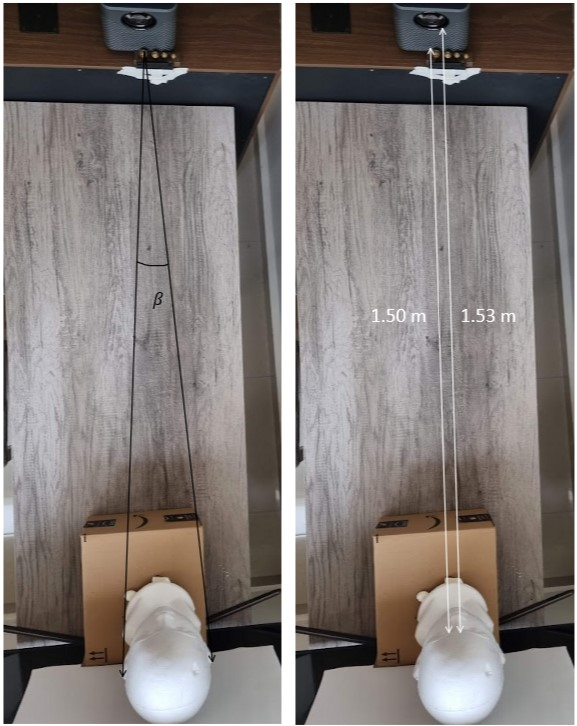
\includegraphics[width=0.3\textwidth, angle =90]{Figures/Exp_Setup.jpg}
    \caption{Experimental Setup}
    \label{fig:Exp_Setup}
\end{figure}

The experimental layout was also designed with the purpose of reducing light noise from the ambient while keeping a clear image free from inside noise caused by the reflection and deformations of the background. This was achieved by covering the top and sides of the setup and by stretching the white background to remove most irregularities on the surface. The background and bust selected for this purpose were both matte white in hopes to reduce the reflective interference to its minimum. \\


\subsection{SURFACE RECONSTRUCTION}
The first step in our method is to obtain the phase of the system. The team used equation \ref{eq:phase} to implement a script that is given the pictures $I_n$ and returns a matrix with the phase values at each point. This phase matrix is visualized in figure \ref{fig:Wrapped_Phase} (b).  

\begin{figure} [H]
     \centering
     \begin{subfigure}[b]{0.22\textwidth}
         \centering
         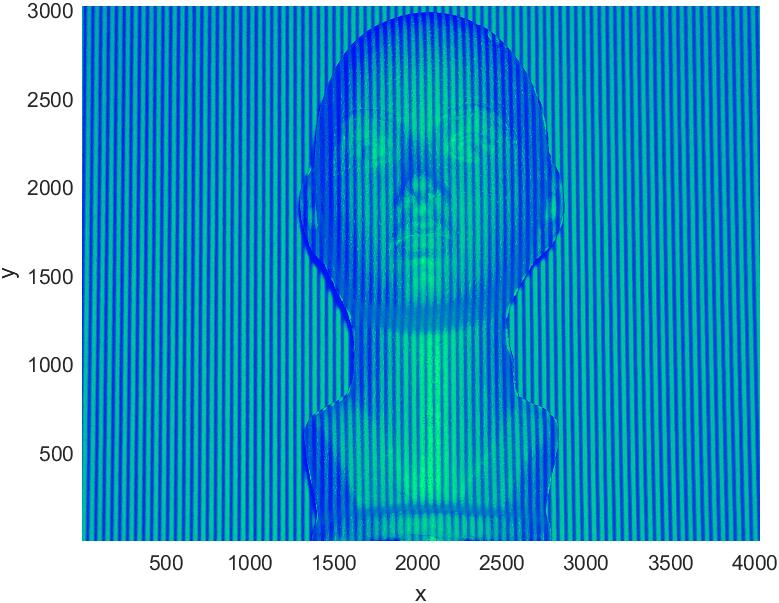
\includegraphics[width=\textwidth]{Figures/Fringe_Imaging.jpg}
         \caption{Fringe Imaging $I_n$}
         \label{fig:Fringe_Imaging}
     \end{subfigure}
     \hfill
     \begin{subfigure}[b]{0.22\textwidth}
         \centering
         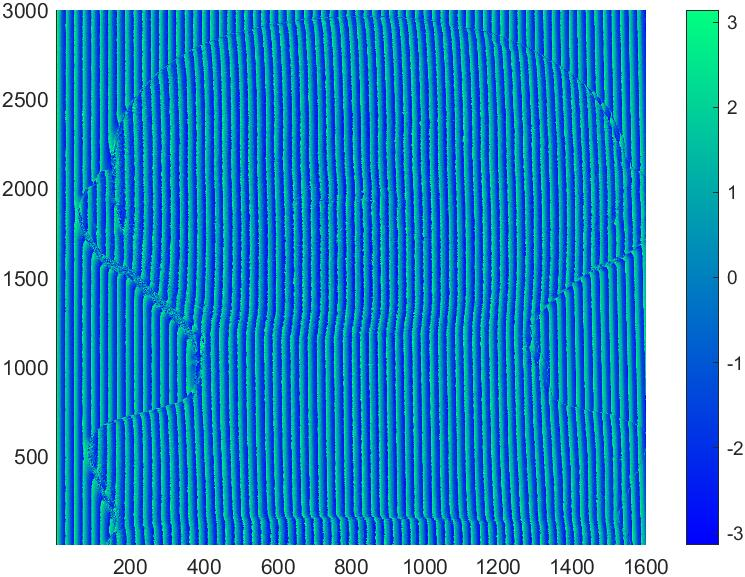
\includegraphics[width=\textwidth]{Figures/Wrapped_Phase.jpg}
         \caption{Phase (Wrapped)}
     \end{subfigure}
        \caption{Phase Measurement}
        \label{fig:Wrapped_Phase}
\end{figure}

After we obtained the wrapped phase of the system, the team used a series of processing algorithms to extract the three dimensional measurements of the object. As discussed in section \ref{sec:TEO_FRAMEWORK}, the phase unwrapping algorithm is critical. %COMO SE LLAMA Y CITA????%%%%%%%%%. 
Unwrapping the phase lead to a result that resembles the object but is tilted as shown in figure \ref{fig:Unwrap_Phase}.

\begin{figure}[H]
    \centering
    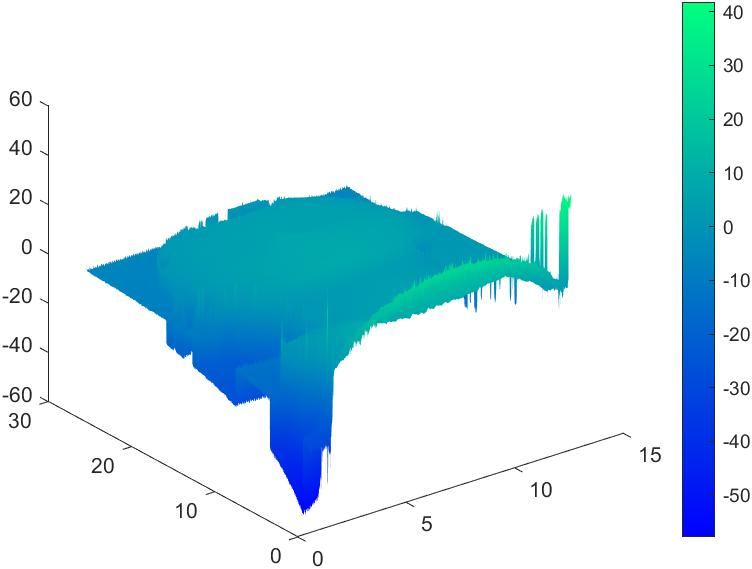
\includegraphics[width=0.2\textwidth]{Figures/Unwrap_Phase.jpg}
    \caption{Unwrapped Phase}
    \label{fig:Unwrap_Phase}
\end{figure}

 The team later related the unwrapped result to the z measurement with equation \ref{eq:topography}. To this result we call the topography of the bust and its also stored in a matrix format. After implementing a numeric filter to smooth the data, the results are the following (Figure \ref{fig:TopBust}):

\begin{figure}[H]
    \centering
    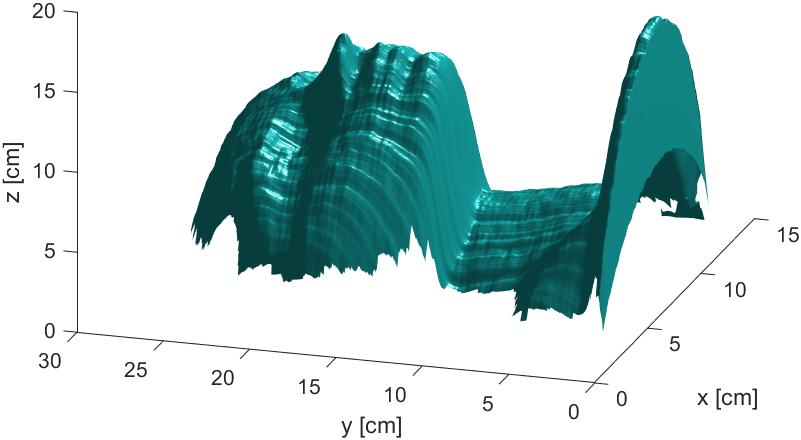
\includegraphics[width=0.4\textwidth]{Figures/Bust_Face.jpg}
    \caption{Topography of the bust}
    \label{fig:TopBust}
\end{figure}

Table 1 shows the quantitative measurements of the bust. From this data the team reports that the measurements deviate from the real value by 0.19 [cm]. This corresponds to a 1.1 $\%$ of relative error. 

\begin{table}[H]
\resizebox{\columnwidth}{!}{ % Scale to column width
\begin{tabular}{|l|l|l|}
\hline
                             & \textbf{Ear to Ear}    & \textbf{Back to Nose}     \\ \hline
Real Value                   & 14.2 {[}cm{]} & 16.4 {[}cm{]}    \\ \hline
Moire by Fringe Displacement & 13 {[}cm{]}   & 16.5937 {[}cm{]} \\ \hline
\end{tabular}
}
\label{tab:Measure}
\caption{Measurements of the Bust}
\end{table}

%Alternative method for 360° scanning
%We tried to implement an alternative for the two mirror 360° \(buscar la referencia del dr rayas) scanning method by rotating the object and dividing it in four sections.
%Esto sería conclusión?

%Four side scanning
%Matrix Superposition Method: hacer un surf con un hold on. (Unir los 4 scans)
%Suavizado

After obtaining the unwrapped, filtered and adjusted reconstruction of each side of the bust the team used a matrix superposition method in which it used the different parts of the simulated mannequin to reconstruct the whole bust. This matrix superposition consists on adjusting the matrix data of each side to be compatible in a single simulation so that each scanned side can fit its designated position. Two variations of this method were applied differing only in the computational simplicity and the exactitude of the final product. \\

\subsubsection{DOUBLE MATRIX RECONSTRUCTION}
%Cabeza back-front 
%Cabeza side1-side2
%Discución de la comparación de ambos resultados
The first variation of the matrix superposition method is called the double matrix reconstruction or two-face reconstruction. This method consists in using the front face and the back of the head of the simulated bust. Both halves would then be adjusted in their spatial position to fit with each other. \\

%%IMAGE OF DOUBLE SIDE RECONS
\begin{figure}[H]
    \centering
    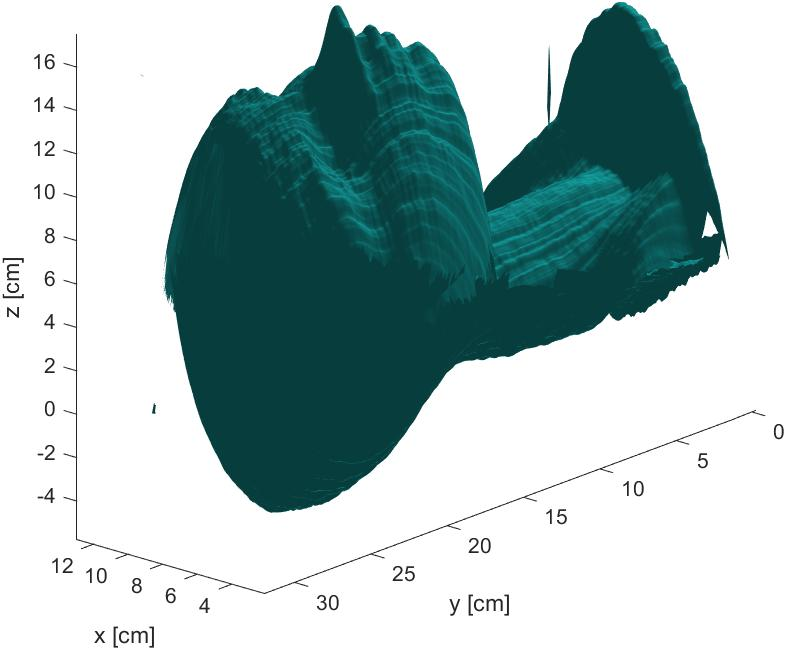
\includegraphics[width=0.35\textwidth]{Figures/Bust_Face_Sidejpg.jpg}
    \caption{Reconstruction using the front and back face of the bust}
    \label{fig:Double}
\end{figure}

The advantage of using only the front and back side of the bust is the simplicity of the reconstruction. In this case the detail on the sides of the bust where not completely lost in the double matrix reconstruction, as seen in figure \ref{fig:Double}, which is fortunate for this simulation. Almost no adjustments were needed to fit both sides together as they were already aligned in the experiment. There was a slight variation in height between the faces due to a deformity in the base of the bust which caused its forward inclination to change when it was rotated. The only disadvantage of this method is that it may loose accuracy in the sides of the reconstructed object. If the object that is scanned is symmetrical or has little to no imperative details on the sides then this method is ideal. \\

\subsubsection{QUADRUPLE MATRIX RECONSTRUCTION}
Countering the double matrix reconstruction discussed earlier, the team came up with the quadruple matrix reconstruction or four-face reconstruction. This method, similar to its counterpart, adjusts the scanned reconstructions of the object in space to make them compatible in a simulation. The quadruple matrix reconstruction uses four scanned sides of the object to offer a more accurate reconstruction of the object. Apart from using the front side and the back side of the object like its homologue, this method implements the lateral sides of the object to bring a more detail to the sides than the double matrix reconstruction method. In figure \ref{fig:Quadruple}, we can see the added detail of the ears in the simulation. \\

%%IMAGE FOUR SIDE RECONS
\begin{figure}[H]
    \centering
    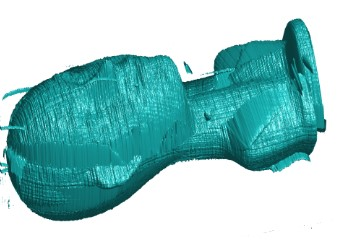
\includegraphics[width=0.35\textwidth]{Figures/FourSideRecons.jpg}
    \caption{Reconstruction using the front, back, left and right sides of the bust}
    \label{fig:Quadruple}
\end{figure}

It is true that this method offers a more precise reconstruction of the original object as it take into account more sections of the same. The principal disadvantages the team found with this method is that the spatial adjustment of the position of the four sides is very complicated using the current tools. The human error made when rotating the object is clearly visible while using this method as the slightest error in the scan can lead to a visible deformity in the simulation. As mentioned before, while processing any side of the object there is noise coming from the background which leads to imperfections in the simulation, this noise and imperfections also collaborate into creating a messy image when combined with the rest of the processed images. If the scanning process gets improved in the future, the four-face reconstruction could prove to be superior than its homologue and there could be even a six-face method where the top and bottom of the object are also implemented into the simulation. \\

\section{Conclusion}
%% NUESTRA PROPUESTA
%Advantages: More clarity by taking into account the four sections.
%Disadvantages: The object (al mover todo el experimento) manipulation may affect the results but this can be changed with a more technical setup.
%Posibles mejoras: buscar unwrappings mas eficientes. un setup profesional que no permita vibraciones ni variaciones en los resultados. Un fondo blanco que sea completamente plano.

%Alternative method for 360° scanning
%We tried to implement an alternative for the two mirror 360° \(buscar la referencia del dr rayas) scanning method by rotating the object and dividing it in four sections.
%Esto sería conclusión?

%% REPORTAR LAS POSIBLES APLICACIONES DENTRO DE LAS AREAS QUE MENCIONAMOS EN LA INTRODUCCION.

The three dimensional reconstruction with the double and quadruple matrix reconstruction proved to be a viable approach to obtain an accurate digital model of an object. Its simplicity lies in the scanning process which is straight forward and does not require major measurements to set up. By dividing the object into major sections and then scanning side sections individually the team was able to add the individual pieces into one complete figure as in a simple puzzle. \\

This method was developed as an alternative for other 360° scans like "3D shape and strain measurement of a thin-walled elastic cylinder using fringe projection profilometry" by Antonio de Jesús Ortiz-González, Amalia Martínez-García, Juan Benito Pascual-Francisco, Juan Antonio Rayas-Álvarez, and Alexis de Jesús Flores-García \cite{de20213d}. The target of the matrix reconstruction variations was to create an easier way to set the experiment up with less specialized materials while guaranteeing precise results. \\

The major issue with the matrix reconstruction variations comes from the need to guarantee that the object stays in the same position when rotated to minimize errors. This could be improved by finding a symmetrical axis in which the object could be rotated without being removed from the base. An important consideration from this method is to take into account the symmetry of the object to define which sides should be scanned and how many sections should the object be divided into. For the reconstruction itself, the main adjustments the team missed to implement due to the time constraints were the noise cleansing of the simulation and the spatial positioning of the different pieces. \\

An important remark the team realized with this experiment is that while using the matrix reconstruction method variations it is easier to obtain clearer images when using the least amount of pieces of the object while sacrificing detail. If the user wishes to obtain a clearer image then it is advised to use a greater number of images while having in mind that the clarity of the reconstruction might be compromised if not executed in an ideal way. As an additional note, the team would like to recommend using an even number of sections from the object to ease the simulation setup. \\

Further improvements include using a stress free background to reduce noise in the simulations. This can be achieved by using a sturdier material which is immune to deformities. The setup could also be further improved to be invulnerable to vibrations removing the fear of interacting with the objects conforming the setup. The wrapping method could be improved by using a Fourier method rather than equation \ref{eq:phase}. Furthermore, there may be more efficient unwrapping methods that could reduce the computational time and render better results. \\

This method could be implemented in a variety of fields from the medical imaging of superficial tissue or limbs to create adapted prostheses to the fashion industry when scanning body parts to create tailor made clothes and accessories fit for the client. In paleontology and archaeology a fringe scanning and matrix reconstruction method could allow researchers to create a model to analyze details of a desired object without fear of damaging the object by manipulating it. The possibilities to apply this method in different industries seem endless which makes improvements to this method necessary to be more adaptive to different circumstances.


% References
\printbibliography

\end{document}